\documentclass[11pt]{article}
\usepackage[margin=1in]{geometry}
\usepackage[parfill]{parskip}
\usepackage{amsmath, amsfonts,tabularx,graphicx, subfigure}
\title{Improving the Performance of Distributed Data Parallelism \\Over a Low Bandwidth}
\author{Christopher Rae \\ \begin{small} email: raecd123@gmail.com \end{small}}

\date{}

\newcommand{\textify}[1]{\text{\begin{scriptsize}#1\end{scriptsize}}}

\begin{document}
\maketitle


\begin{abstract}
There is no doubt that networking is a bottleneck when training neural networks across multiple GPUs and computers. Having a low bandwidth or a high latency can drastically increase training time of a neural network. In this paper we look at a variety of methods to reduce the effect of a low bandwidth including gradient sparsification, gradient quantization and a using a large batch size. We find ... COULDN'T FIND COMPUTER
\end{abstract}
\tableofcontents
\newpage

\section{Introduction}
Distributed data parallelism is a widely used technique for training artificial intelligence (AI) models, especially when working with large datasets. It involves dividing the data across multiple nodes and training multiple copies of the model in parallel, which can significantly reduce the time required for training. However, the efficiency of this technique can be affected by several factors, including the bandwidth of the communication channels between the nodes.

Low WiFi bandwidths can have a significant impact on the training time of AI models using distributed data parallelism. When the communication channels between nodes have low bandwidth, it can lead to slower data transfer and synchronization between the nodes, which can result in slower training times. In addition, low WiFi bandwidths may also lead to increased latency in the communication between nodes, further diminishing the efficiency of the training process.

In this paper, we aim to explore the relationship between low WiFi bandwidths and the training time of AI models using distributed data parallelism. We will discuss the various ways in which low WiFi bandwidths can impact the communication between nodes and the overall efficiency of the training process. We will also present potential solutions for mitigating the negative effects of low WiFi bandwidths on model training time.

To provide a better understanding of the role that WiFi bandwidth plays in the training of AI models using distributed data parallelism, we will conduct experiments using a variety of datasets and model architectures. We will compare the training time of models trained using distributed data parallelism in high and low WiFi bandwidth environments to evaluate the impact of low WiFi bandwidths on the training process.

Overall, our goal is to shed light on the importance of WiFi bandwidth in the training of AI models using distributed data parallelism and to identify strategies for optimizing the training process in low bandwidth environments. We hope that the findings of this research will be useful for practitioners seeking to improve the efficiency of their model training process and for researchers studying the optimization of distributed data parallelism for AI model training.

\section{Methodology}
\subsection{Distributed Data Parallelism}
The goal of distributed data parallelism is to split the data across the GPUs and computers in the cluster, so that the training process can be completed faster by leveraging the additional computational resources.

Here is an overview of the process:

\begin{enumerate}
	\item First, the data and model are partitioned or "split" across the GPUs and computers in 			  the cluster. This is typically done by dividing the data into smaller chunks and 	  				   assigning each chunk to a GPU or computer in the cluster.
	\item Next, the training process begins. On each GPU or computer in the cluster, the model 				  processes the data assigned to it and computes the gradients of the loss function with 		  respect to the model parameters.
	\newpage
	\item The gradients computed on each GPU or computer are then averaged together, and the 				  model parameters are updated using this average gradient. This process is known as 				  "gradient averaging" or "gradient synchronization."
	\item The process is then repeated, with each GPU or computer processing its assigned data 				  and computing gradients, until the model has been trained.
\end{enumerate}

By training the model in this way, the computation is distributed across multiple GPUs and computers, which can significantly reduce the time it takes to train the model. However, it also adds complexity to the training process, as the gradients must be averaged across the GPUs and computers and the model parameters must be kept consistent across the cluster. There are multiple ways of preforming this gradient averaging depending on the architecture of your GPUs and computers. In this paper we work with a synchronous architecture for simplicity and as all of our GPUs have roughly the same compute power. There is also the argument of a centralised versus a decentralised topology.

In a centralized topology, the process of gradient averaging or gradient synchronization in step 3 of the distributed data parallelism process is typically performed on a central server or "parameter server." This is done by sending the gradients computed on each GPU or computer in the cluster to the central server, where they are averaged together and the model parameters are updated.

In a decentralized topology, the process of gradient averaging or gradient synchronization is performed in a decentralized manner, without the use of a central server or parameter server. This can be done using a number of different techniques, such as peer-to-peer communication or gossip protocols.

We find in this paper ---INSERT LINK--- that decentralized topology's are effected less by low bandwidths, and that is why we implement a decentralized architecture in our paper. To be more specific, we use our own implementation of the Baidu Ring AllReduce algorithm to average our gradients.

\subsection{SGD}

The training data is denoted as $\{x_i\}^n_{i=1} \subset \mathbb{R}^d$, and the model parameter vector is donated as\\ $w \in \mathbb{R}^d$. The goal of training is to solve the following optimization problem 
$$
\min_w f
(w) = \frac{1}{n} \sum^n_{i=1}L(w,x_i)
$$
Where $L$ is the loss function. We typically use an algorithm such as stochastic gradient descent(SGD) to solve the equation above. In which we need to calculate the unbiased stochastic gradients of $f$ at time step $t$ which satisfies $\mathbb{E}[g_t(w)] = {\nabla} L_t(w)$. SGD can be written as:

$$
w_{t+1} = w_t - \eta g_t(w_t)
$$

Where $g_t(w_t)$ is an estimate for the actual gradient ${\nabla} L_t(w_t)$ and $\eta$ is the learning rate. For simplicity we'll let $g$ represent $g_t(w_t)$. The convergence of SGD is largely influenced by the variance of $g$. In most implementations of distributed parallelism it is $g$ which is averaged between all of the replicas.


\subsection{Gradient Quantization}
Gradient quantization is a technique used in distributed data parallelism to reduce the amount of data that needs to be transmitted over channels during training. It works by reducing the precision of the gradients that are transmitted between worker nodes.

A model parameter is usually stored in memory as a 32bit floating point. There are $7, 800, 000, 000,\\ 000, 000,000,000,000,000,000,000,000,000,000,000,000,000,000$(38zeros) unique 32bit floating points, but that said 32bit floating points like $0.000100$, $0.000101$ and $0.000102$ are very close. We can approximate these numbers to be equal, this is the core concept of quantization.

If you have a vector $a \in \mathbb{R}^d$ where $a \sim \mathcal{N}(0.1,0.55)$ where we know the $\max a$ and $\min a$. We can split $a$ into equal size bins and represent each bin with either a 8bit or 16bit integer. For example, suppose we have a set of 100 bins, each representing a range of gradient values. If the gradient of a particular parameter falls within the range of the first bin, it will be represented as a 1; if it falls within the range of the second bin, it will be represented as a 2; and so on. Then once the quantized $a$ has been sent to another node that node can look up what values the bin represents and replaces all the gradients in the bin with that value. This allows us to represent each gradient value using a single integer, rather than a floating-point value, which can significantly reduce the amount of bandwidth required to when sending gradients. The difference between using 8bit or 16bit integer is the number of bins, which effect not only the accuracy of the data but how much data is sent over the network. If we use 16 bit integers there can be 65,536 bins where as with 8bit there is only 256 which is a significant reduction.

\subsubsection{Non-Linear Quantization}

As mentioned above $a \sim \mathcal{N}(0.1,0.55)$ this tells us that that most of the values will be located around $0.1$ which means it may be more representative of $a$ if the there are more bins located around the mean than $\max a$ and $\min a$ so bins near the mean cover a lower range of values meaning they are occur at a higher frequency, bins closer to the min and the max cover a larger range of values. Instead of all the bins covering an equal range of values at a common interval each bin will contain an equal range of values(if you have 200 gradients and 10 bins each bin will contain 20 gradients). This value assigned to the the bin is the mean of the values in the bin.

\subsubsection{Block-Wise Quantization}

Modern models can contain billions of trainable parameters, which translates to billions of gradients. If we represent all of those gradient as 256 different integers we loose a lot of accuracy and make it alot harder for the model to converge, so what we do is we split gradients into chunks of around 2000 or 4000 items(depending on the size of the model) and quantize each chunk separately this means that the first bin in the first chunk might cover a different ranges of values to the first bin in the second chunk. there are a few reasons for this, the first being that it allows us to use 8bit integers without a significant loss in accuracy, the second being that we can allocate each chunk to a specific GPU core makeing the quantization step a lot faster. If one of the values in $a$ was $7$ it is a clear outlier, this will effect one of the bins causing 1 bin to be wasted because of single outlier. By splitting up the data into chunks only a one of chunks would be effected by this outliers.


\subsection{Gradient Sparsification}
Gradient sparsification is a technique that involves identifying and removing "zero" or nearly zero gradients from the gradients being transmitted between GPUs or computers in a distributed data parallelism setting. The goal is to reduce the size of the gradients without significantly affecting their quality, so that they can be transmitted more efficiently over the network.

In order to perform gradient sparsification we have to decide on a threshold to determine whether or not a gradient is a zero gradient or not, if the gradient is less than the threshold then it it deemed a zero gradient. In our implementation of gradient sparsification we accumulate zero gradients locally and sum them with gradients from the next iteration. 

\subsubsection{Formula}
We denote sparsified gradients as $S(g, Z_t)$. We have to remember that $g \in \mathbb{R}^d$ so we let $g_i$ be the $i$-th component of the vector ($g=[g_1,\ldots,g_d]$). $Z \in \mathbb{R}^d$ is a vector with the same shape a $g$, when the $w$ is initialized at the start of the training process $Z_{0,i} = 0$. The function $S$ has 2 outputs the first being $v$ the new representation of the gradient of the weights at iteration $t$, and the second being the accumulated gradients $Z_{t+1}$

Sparsification of the gradients is shown as follows: 
$$
v_{t,i} =
\left\{
	\begin{array}{cc}
		0 & \quad \left| g_i + Z_{t,i}\right| < \alpha \\
		g_i + Z_{t,i} & \quad \left| g_i + Z_{t,i}\right| \geq \alpha
	\end{array}
\right\}
$$
$$
Z_{t+1,i} =
\left\{
	\begin{array}{cc}
		Z_{t,i} + g_i & \quad \left| g_i + Z_{t,i}\right| < \alpha \\
		0	& \quad \left| g_i + Z_{t,i}\right| \geq \alpha
	\end{array}
\right\}
$$

where $\alpha$ is the the threshold.


\subsection{Larger Batch Sizes}
In machine learning, the batch size refers to the number of samples that will be processed before the model's weights are updated. The batch size is a hyper parameter that can be chosen when training a model. When using a batch size the SGD algorithm becomes mini-batch SGD it looks something like this:

$$
g = \frac{1}{B_k} \sum_{i=1}^{B_k} {\nabla} L(w_t)
$$
$$
w_{t+1} = w_t - \eta g
$$ 


Where $B_k$ is the batch size. Increasing the batch size in a distributed training setup can also improve training efficiency by reducing the frequency of the gradient averaging step. This is because each device will process a larger amount of data before the gradients are averaged and applied to the model weights. This can reduce the overhead associated with performing the gradient averaging step, and can allow the model to make more efficient use of the available computation resources.

One negative effect of large batch sizes is that they can lead to a decrease in generalization performance. This occurs because large batch sizes can result in an increase in the variance of the stochastic gradient descent (SGD) updates, which can cause the model to overfit to the training data. This overfitting can manifest as a decrease in performance on held-out test data or a decrease in the ability of the model to generalize to unseen data.

Another negative effect of large batch sizes is that they can lead to a decrease in the convergence rate of the model. This occurs because large batch sizes can result in a reduction in the magnitude of the SGD updates, which can slow down the convergence of the model. In some cases, this can result in the model failing to converge at all.

Furthermore, using large batch sizes can lead to an increase in the amount of memory required to store and process the data. This can be a problem for systems with limited memory or for models with a large number of parameters, as the large batch sizes may not fit in memory.

One way to counteract the second point is to increase the learning rate $\eta$ so that the magnitude of the SGD updates are increased this usually works for a few of epochs but after a while has a limited effect. We plan to use a dynamic batch size. At the start of training a an initial batch size is determined, and the primary test error is calculated from the models untrained parameters. After each epoch the the the test error is checked, once the test error is half of the primary test error the batch size gets doubled, once the test error is a quarter of the primary test error the batch size is doubled again batch.

Another way which we can reduce the negative effect of a large batch size is to use a different optimizer algorithm to SGD A common choice is Adam (Adaptive Moment Estimation) but adam has been found to scale poorly with large batch sizes. There are 2 optimizers that scale well with large batch sizes, LARS (Layer-wise Adaptive Rate Scaling) \& LAMB (Layer-wise Adaptive Moments for Batch Training)



\iffalse
such as Adam. Adam (Adaptive Moment Estimation) is an optimization algorithm. It is an extension of the stochastic gradient descent (SGD) algorithm and combines the benefits of SGD with the benefits of other adaptive optimization algorithms such as RMSprop. 

One way that Adam helps to reduce the negative effects of using a large batch size is by using an adaptive learning rate. Adam maintains an exponential moving average of the gradients and the squared gradients, which it uses to compute an adaptive learning rate for each parameter. This adaptive learning rate is then used to update the parameters of the model, rather than using a fixed learning rate as in SGD. 

By using an adaptive learning rate, Adam is able to make more aggressive updates to the model's parameters when the gradients are small and make smaller updates when the gradients are large. This can help the model converge more quickly and reduce the negative effects of using a large batch size.
 
In addition to using an adaptive learning rate, Adam also incorporates momentum into the optimization process. This helps the model to continue making progress even when it encounters noisy or oscillating gradients although this doesn't have an effect on the low bandwidth.
\fi



\subsubsection{Formula for the Dynamic Batch Size}

Let $E_e$ be the test error function at epoch $e$ which takes the parameters $w_t$ which is the model parameters at the time step $t$ at the start of epoch $e$. Let $b$ be the initial batch size and where      $\beta$ is the maximum batch size.  

\begingroup
\Large
$$
\varepsilon = \max \left(1, 2^{(\lfloor E_0(w_0,x_R)/E_e(w_t, x_R) \rfloor -1)} \right)
$$
$$
B_k = \min \left(\beta,b\varepsilon\right)
$$
\endgroup

These equation explain dynamic batch sizing. First the scaling factor $\varepsilon$ where $E_0(w_0,x_R)$ is the primary test error, we make sure that value of $\varepsilon$ is greater than 1 as if for some reason $E_0(w_0,x_R) < E_e(w_t, x_R)$ the batch size would decrease which is not what we want. Then its just a case of multiplying $b$ by your scaling factor $\varepsilon$ and checking to see if its greater than $\beta$. Please not that using the output of a loss function in stead of the test error is sufficient.


\subsection{Models}
Within our test we use a range of different models. The most important factor when choosing a model is to make sure we get a good range of sizes between out models. These are the models we have tested:

\begin{center}
\begin{tabular}{| p{3cm} | p{3cm} | p{3cm} | p{3cm} |} 
\hline
Model & No. Parameters &  Gradient Physical Size (MB)\\ \hline
RESNET-50 & 25,583,592 &  94.1 \\ \hline
VGG16 &  138,357,544 &  428.2 \\ \hline
Inception v4 & 42,608,450 &  170.2\\ \hline
%Transformer & 0 & Multiple & GLUE \\ \hline
%RoBERTa-Large & 0 & Multiple & GLUE \\ \hline
\end{tabular}
\end{center}


\section{Results}
We start by calculating a theoretical minimum training time. 
\begin{figure}[h]
  \centering
  \subfigure[\begin{small}Training 1 Epoch on 1 P100 GPU \end{small}]{
  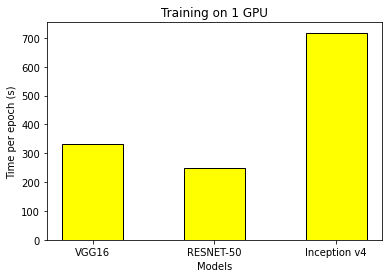
\includegraphics[width=6cm]{models.png}
  }
  \subfigure[ The Theoretical Time to Send Gradients]{
  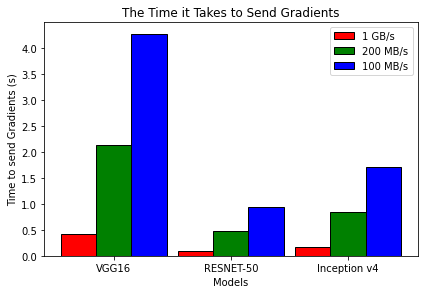
\includegraphics[width=6cm]{gradientTimes.png}  
  }
  \caption{\begin{small} a \& b \end{small}}
\end{figure}

In an ideal world training speed would increase linearly with the number of GPUs you have training the model. In our test to determine the results of Figure 1 (a) we train each model with a $B_k$ (batch size) of 32 and on the cifar 100 dataset of which we use 50000 images for training, this means that there are just under 1600 iterations in a single epoch. Figure 1(b) is determined by the size of the model divided by the speed of the network.

\subsection{8 GPUs Theoretical}
In out result we plan to compare the theoretical with the applied.In this case 8 GPUs were each node has 1 GPU, the data is evenly split between each node translating to each node training with a sample of 6250 images. By increasing the number of nodes from 1 to 8 we reduces the number of communication steps per epoch(and iterations) to around 200 but there is also more data sent in each communication step as each node is sending its own gradients to 8 other nodes. 

If each node was to individually send its gradients to all the other node, there would be 56 ($N(N-1)$ where $N$ is the number of nodes) separate messages sent between nodes, if we were dealing with the worst case scenario where you are training VGG16 on 100MBps you would have around 4 minutes of communication per epoch. This is cause by only 1 node sending data at a time while the rest of the nodes are idol caused by the networks constraints. As we are using a more efficient ring all reduce algorithm, we should have communication times similar to what is shown in Figure 1 (b)

We plan to use 8bit quantization using both non-linear and block-wise techniques. non-linear quantization doesn't effect bandwidth it just helps to reduce variance. Block-wise allows us to decrease the gradients size by a factor of 4 but adds $\frac{p}{k}\times 256$ float16 numbers on top of the quantized gradients in order to undo the quantization where $p$ is the number of parameters and $k$ is the value that determines the number of block usually 2048 or 4096. For the example of vgg16 you decrease the gradients to around 110 MB in size but add an extra size of 8,000,000 32 bit floating points.

When using sparsification with quantization, sparsification occurs before quantization and quantization only occurs on the non zero grads.

\begin{figure}[h]
	\centering
	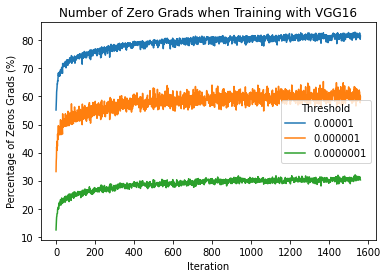
\includegraphics[width=7cm]{zeroGrads.png}
	\caption{\begin{small} Percentage of Zeros Grads in the First Epoch\end{small}}
\end{figure}

We see that as the model gets closer to converging the number of zero grads increases, the graph also shows us that when we have a threshold of 0.00001 we drop over 80\% of our gradients this seems like it would have a large effect on the training process this is something we will address in our applied section of the results. If we drop 80\% that would also mean you are only sending 20\% of gradients being sent between nodes over the network, on a network with a low bandwidth.

By doubling the batch size you should half the communication time as there half as many communication step taking place in an epoch. Whilst using a dynamic batch size it can take quite a long time before the batch size doubles as the it takes multiple epoch before the train error halves.


\subsection{8 GPUS Applied}
\begin{Huge}
\begin{center}
COULD NOT ACCESS A COMPUTER
\end{center}
\end{Huge}


\section{Conclusion}
 

\end{document}